\begin{figure}[!htb]
\centering
    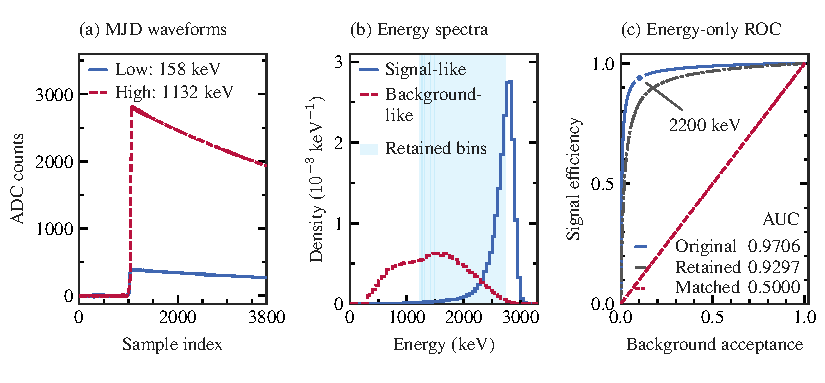
\includegraphics[width=\linewidth]{wing_contribution/figures/mjd_motivation_main_v2_generated.pdf}
\caption{Energy shortcuts in detector data.
(a) Baseline-subtracted MJD waveforms from two clean test events with energies of 158 and 1132\,keV.
(b) Unit-area energy spectra for SuperNEMO $0\nu\beta\beta$ (signal-like) and $^{214}$Bi (background-like) test events. Shading marks retained 5\,keV matching bins; spectra use 50\,keV display bins.
(c) ROC curves using energy alone as the score for the original population, retained events with unit weights, and the same retained events after matching. The point marks a 2200\,keV threshold.}
\label{fig:mjd-motivation}
\end{figure}
